\chapter{Gruppenfilter}\label{gruppenfilter}
\begin{figure}[h!]
	\centering
	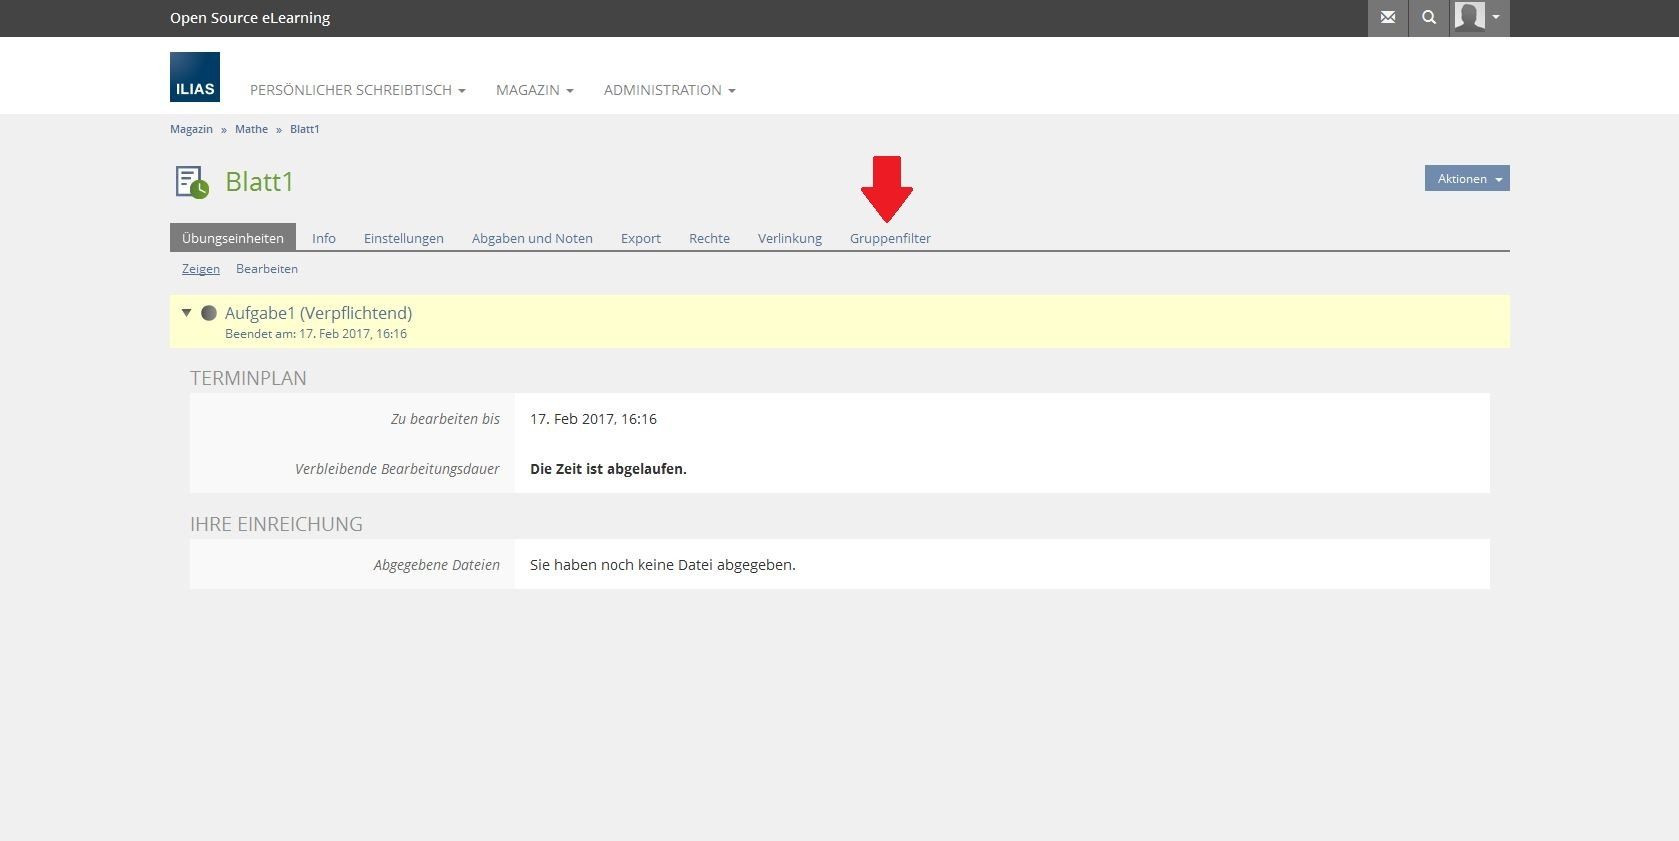
\includegraphics[width=1\textwidth]{img/excerciseGruppenfilter.jpg}
	\caption{Ansicht Gruppenfilter Tab}
\end{figure}

Text wo finde ich den Tab
\newpage
\section{Gruppenfilter}
\begin{figure}[h!]
	\centering
	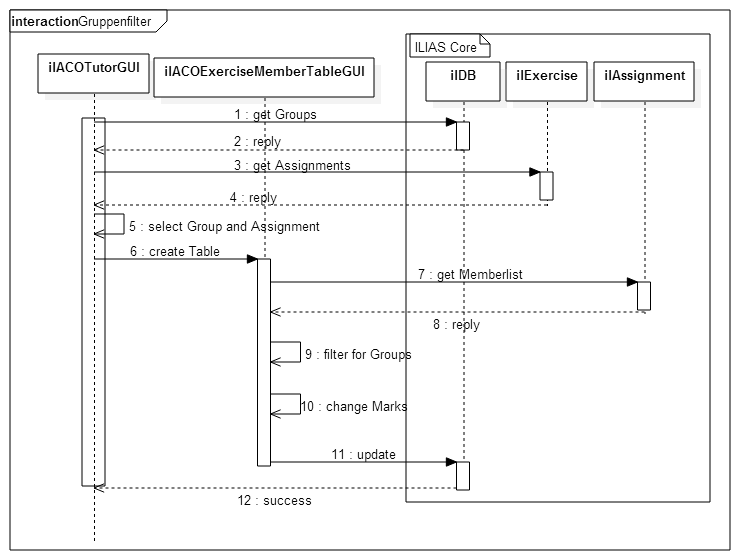
\includegraphics[width=.7\textwidth]{img/seq_tutorGUI.png}
	\caption{Sequenzdiagramm Gruppenfilter}
\end{figure}
\begin{figure}[h!]
	\centering
	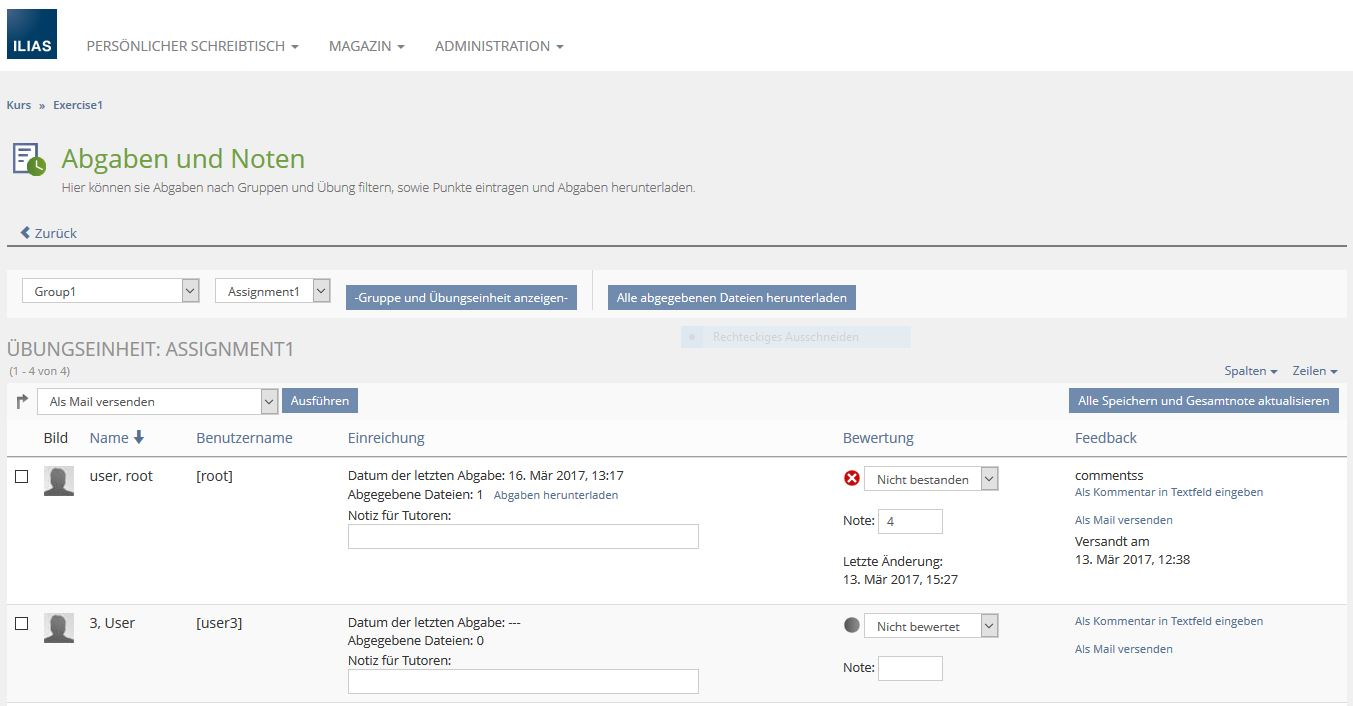
\includegraphics[width=1\textwidth]{img/excerciseGruppentabelle.jpg}
	\caption{Ansicht Gruppenfilter Tabelle}
\end{figure}
~\\Innerhalb von Excercises bzw. Übungen erscheint dieser Reiter/Tab, der es ermöglicht Abgaben nach Gruppen zu filtern. 


\subsection*{Unterpunkt}
\begin{itemize}
	\item Text Unterpunkt
\end{itemize}

\clearpage